\documentclass{sig-alternate}

\usepackage{array}
\usepackage{pifont}
\usepackage{url}
\usepackage{graphicx}
\usepackage{multirow}

\newcommand{\none}{\ding{55}}
\newcommand{\least}{\ding{51}}
\newcommand{\little}{\ding{51}\ding{51}}
\newcommand{\lots}{\ding{51}\ding{51}\ding{51}}


\begin{document}
\pagenumbering{arabic}


\title{Cheminformatics: The Computer Science of Chemical Discovery}
\numberofauthors{9}
\author{
\alignauthor
Joerg Kurt Wegner\\
       \affaddr{Tibotec BVBA}\\
       \affaddr{Turnhoutseweg 30}\\
       \affaddr{2340 Beerse Turnhout, Belgium}\\
       \email{jwegner@its.jnj.com}
% 2nd. author
\alignauthor
Aaron Sterling\\
       \affaddr{Department of Computer Science}\\
       \affaddr{Iowa State University}\\
       \affaddr{Ames, Iowa, USA}\\
       \email{sterling@iastate.edu}
% 3rd author
\alignauthor
Rajarshi Guha\\
\affaddr{NIH Center for Translational Therapeutics}\\
\affaddr{9800 Medical Center Drive}\\
\affaddr{Rockville, MD 20850}\\
\email{guhar@mail.nih.gov}
}

\additionalauthors{Additional authors:
Andreas Bender (University of Cambridge, email: {\texttt{andreas.bender@cantab.net}}),
Jean-Loup Faulon (University of Evry, email: {\texttt{Jean-Loup.Faulon@issb.genopole.fr}}),
Janna Hastings (European Bioinformatics Institute, Cambridge, UK, email: {\texttt{janna.hastings@gmail.com}}),
Noel O'Boyle (University College Cork, Cork, Ireland, email: {\texttt{baoilleach@gmail.com}}),
John Overington (European Bioinformatics Institute, Cambridge, UK, email: {\texttt{jpo@ebi.ac.uk}}),
Herman Van Vlijmen (Tibotec, Beerse, Belgium, email: {\texttt{hvvlijme@its.jnj.com}}), and
Egon Willighagen (Karolinska Institutet, Stockholm, Sweden, email: {\texttt{egon.willighagen@ki.se}})
.}
\date{25 June 2011}


\maketitle
\begin{abstract}
  One of the most prominent success stories in all the sciences over
  the last decade has been the advance of bioinformatics: The
  interdisciplinary collaboration between computer scientists and
  molecular biologists led as one of its major accomplishments to the
  sequencing of the human genome, where researchers connected
  biological concepts to the theory of string algorithms. However,
  despite this great success, few computer scientists are familiar
  with a related discipline: cheminformatics, the use of computers to
  represent the structures of small molecules and analyze their
  properties.  Cheminformatics has wide applicability, from the
  discovery of novel drug candidates to the optimization of certain
  physicochemical properties of small molecules. Until recently, much
  of the the data and some of the techniques employed in the
  cheminformatics field have been closely guarded secrets of companies
  whose financial success depended on being the first to produce the
  new therapeutic molecules.  Only within the last decade -- and as an
  effect of a change in mindsets, government-mandated policy changes,
  and, not least, because of chemists volunteering their time
  for an Open Science ``movement'' -- have researchers gained access to
  freely available software packages and databases of tens of millions
  of chemicals. Academic chemists now confront a variety of unsolved
  algorithmic problems that could not have been tackled a decade ago,
  but whose solutions are critical to research ranging from
  determining the behavior of small molecules in biological pathways,
  to finding therapies for rare and neglected diseases.
\end{abstract}

\category{J.2}{Computer Applications}{Physical Sciences and Engineering}[Chemistry]
\terms{Algorithms, Design, Human Factors, Theory}
\keywords{cheminformatics, chemoinformatics, graphs, chemistry, databases, knowledge management, open source, open
data}

\section{Is Cheminformatics the New \\Bioinformatics?}

Novel technologies in the life sciences churn out information at an
ever increasing rate -- public data stores such as the one at the
European Bioinformatics Institute (EBI) contain on the order of 10
petabytes of biological information.  While biological information has
been publicly available for decades, the same has not been true for
chemical information, until recently. It was not until 2004 that a
large public small molecule structure repository (PubChem) became
freely available. This was followed by other databases, as discussed
later in this article. While much of the foundational algorithms of
cheminformatics have been described since the 1950s, publically
available software implementing many of these algorithms have only
been accessible in the last ten to fifteen years \cite{faulon2010}.

So why should we actually care about chemical information being made
public -- and how does this relate to the field of computer science?

Making chemical information public is important because the drugs we
take are the result of intensive and costly research, which is
facilitated by the amount of information available. The more
information is shared (a process very hard to achieve in
pharmaceutical companies), the more information is available to each
researcher, facilitating the development of novel treatments. The
relevance of computer science to this research becomes clear when we
consider the quantity and types of data available -- currently a
single data base such as PubChem contains more than 34 million
chemical structure records, along with an even larger number of
\emph{annotations} (comments on the structure that are database searchable), such as synonyms (different names for the same molecule), known targets (drugs with which the molecule is known to interact), mode of action (how the molecule reacts with others),
regulatory approval status and so on.  Simply considering the synonym
list, PubChem stores 50.1 million synonym for 19.6 million compounds.

The design of data structures for this chemical information, as well
as subsequent data mining of this information, are areas where
expertise in computer science is urgently needed. (For a recent,
detailed introduction to cheminformatics, written for computer
scientists, see \cite{brown2009}).

Cheminformatics comprises different areas, which broadly speaking can
be divided into three fields: \emph{capturing data} (using lab
notebooks or potentially using formats such as the Chemical Markup
Language for publications); \emph{storing data} (designing database
schemas, devising ontologies) and \emph{mining data} (such as for
bioactivity prediction, which might involve algorithms based on
graphs).  However, the type of information being analyzed is different
from biological information: while bioinformatics often deals with
sequences, the domain of cheminformatics is chemical structures. In
the case of the former, information can very frequently be represented
as one-dimensional strings, which are relatively easy to handle
computationally. In the case of the latter however, chemical
structures may possess rings, branches as well as multiple valid
representations of the same structure (such as \emph{tautomers}, where hydrogen atoms can be positioned in different
places of the molecules), potentially giving rise to
ambiguities. Hence, chemical structures are often reported to be more
difficult to standardize.

To illustrate the difficulty of standardizing chemical structures,
different representations of the same chemical structure are shown in
Figure~\ref{figure:chemical-structures}. The representations range
from a graph (Fig.~\ref{figure:chemical-structures}A) that contains
much implicit information (such as unlabeled nodes represent carbons
with valencies satisified by hydrogens) to a fully labeled graph,
where all information is explicit
(Fig.~\ref{figure:chemical-structures}B). The former is what is
usually exchanged informally between chemists, but to actually mine
chemical structures computationally, something like the latter is
required.  For example, graph mining algorithms can be applied to
labeled graph representations, to discover patterns in large-scale
datasets \cite{horst2009}.

\begin{figure}
\centering
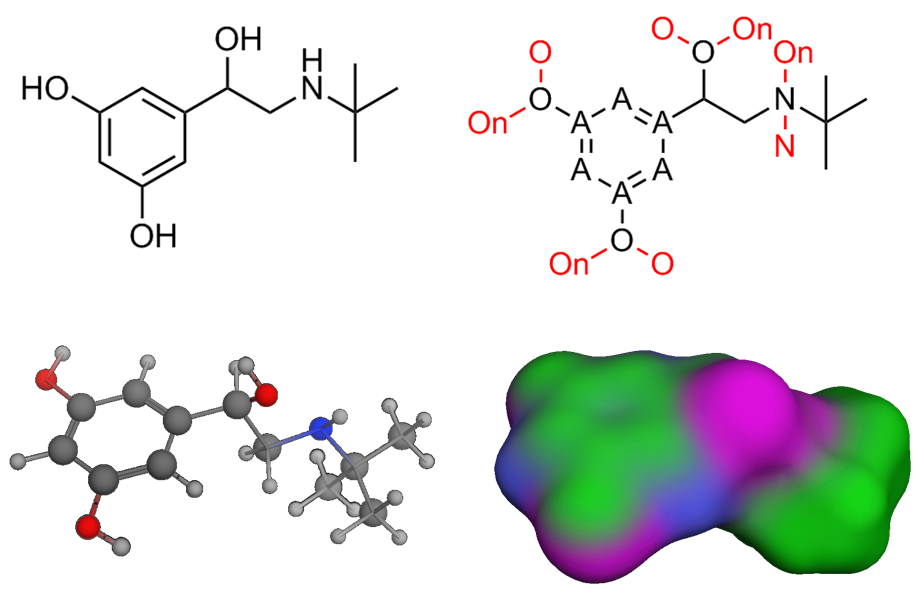
\includegraphics[height=2in]{chemical-structures.png}
\caption{A hierarchy of chemical structure representations, increasing
  in information content from left to right and top to bottom. A
  chemists traditional 2D depiction (A), a labeled graph (B), a 3D
  conformation (C) and a surface represention (D). All show differing
  (and valid) aspects of the same molecule and are suited for
  differing purposes. The choice of representation is guided by the
  intended use of the structure data.}
\label{figure:chemical-structures}
\end{figure}

Although graphs implicitly encode the 3D structure of a molecule
(when combined with knowledge about favored bond angles and
distances), many different low energy 3D structures, or conformers,
may be consistent with the same graph structure. In addition, the 3D
structure may have a ``secondary'' geometrical arrangement of features
(such as the presence of a right-handed helix) which cannnot be
encoded in the graph. Thus we have 3D representations
(Fig.~\ref{figure:chemical-structures}C) that make the 3D arrangement
of atoms and bonds explicit. Fig.~\ref{figure:chemical-structures}D
goes further and represents a molecular surface, encoding some
property (such as lipophilicity, the ability to dissolve in fats) that varies over the surface.

Even though some structure representations contain more explicit
information than others, they are all equally valid and are suited for
different problems. Indeed, Fig.~\ref{figure:chemical-structures}
represents a hierarchy of representations. Thus, when searching for
substructures, a 2D representation is sufficient. When trying to
rationalize why a molecule binds to a protein, a 3D structure is
vital.

Given that a fundamental principle of the field is that \emph{similar
  molecules exhibit similar properties} \cite{Johnson:1990qf}, the
choice of representation is key in determining how such similarities
are evalaued, and thus the effectiveness of subsequent analyses. But
even after one has selected a representation one faces the challenge
of balancing computational costs with the utility of the
representation. For example, a full 3D description of a molecule,
taking into account all possible conformers would let us accurately
predict many properties. But the size of this representation and the
time required to evaluate it would be prohibitive. Instead, can we
obtain accurate predictions from a subset of conformers? Or, can we
obtain comparable accuracy by using a 2D representation? And is so,
what type of labels are required? Currently, many of these questions
are answered using trial and error.

From the above it becomes clear that the nature of chemical problems
is often a complex mixture of combinatorial and continuous
problems. If we oversimplify the nature of chemical structures and
their properties, we can not describe the world around us in
sufficient detail. On the other hand, if we try to encode every detail
(\emph{e.g.}, all possible 3D structures and their properties, all
metabolites of a structure in humans in different tissues), the
complexity of collecting, storing, and mining these data increases
dramatically. For the field of cheminformatics to flourish, we need
closer collaboration between chemists (or, more generally, life
scientists) and computer scientists -- where the former need to be
able to pose their problems in a way relevant for practical
applications; and where the latter are able to devise ways of
capturing, storing, and analyzing chemical data which achieve optimal
balances between the different risks in generalizable encodings and
complexity (space and time). The goals of cheminformatics are to
support better chemical decision making by 1. storing and integrating
data in maintainable ways, 2.  providing enough open standards and
tools so software engineering concepts allow applications and data to
be used across heterogeneous platforms, and 3. mining the many
chemical property spaces in a time- and space-efficient way. We will
discuss all three goals in the following sections.

\section{Bridging Cheminformatics and Computer Science}

Our motivation for this article is to highlight a variety of topics in
cheminformatics where modern CS research could contribute, and
to present the computational and algorithmic problems
that are addressed in the field.

While cheminformatics has a broad applicability, ranging from
agrochemical research and drug discovery to the design of novel
materials, we have chosen to use drug discovery as the context of this
article due to its central relevance for human wellbeing. Given that
the safety of drugs on the market is a key concern both for the
general audience as well as researchers in pharmaceutical companies,
the remainder of this article is structured around the concept of
``risk minimization'' in drug discovery -- the question of how to
minimize the chances of a small molecule failing, due to poor
physical, chemical or biological properties, in the various research
and development stages as a drug candidate, and how to successfully
employ cheminformatics methods in these efforts. As an example, a
molecule must be soluble and show a certain degree of bioavailability
to be considered as drug candidate. In cases where these properties
are poor, a cheminformatics approach can suggest replacement of
certain functional groups, that maintain potency but improve the
solubility and bioavailability.  Table~\ref{table:properties} (in the
Appendix) summarizes a number of properties a drug candidate must
satisfy to be considered therapeutically useful (such as being
appropriately soluble, exhibiting minimal toxicity and being selective
for the intended target) and sketches the role of cheminformatics at
each stage of drug development.
%
\subsection{Representing and Searching Structures}
\label{sec:databases}
%
Most cheminformatics applications rely on large databases of chemical
structures, their properties, and relationships to, \textit{e.g.},
biological targets.  Organizing and maintaining such databases, as
well as searching and clustering similar structures together, are
essential to enable many scientific applications. Yet, each one of
those areas poses its unique computer science challenges.

There is considerable progress in open chemical and bioactivity
databases like ChEMBL and NCBI-PubChem, which are both freely
available and contain in the order of millions (ChEMBL) and tens of
millions (PubChem) of data points each. Still, the integration of
chemical databases with one other remains a challenge, not only due
to the normalization problems in the chemical and bioactivity
landscape, but also due to sheer data volume. One problem is the
annotation with the ``protein targets'' a molecule binds to -- here
dozens of protein and gene identifiers exist, generally without the
availability of a one-to-one mapping from each ontology, which makes
merging databases often a cumbersome exercise.

Given the requirement to ``make sense'' of as much chemical data at
hand as possible, we have to be able to search in complex data, for
example multi-labelled molecular graphs, where graph labels can change from database to database. Hence, we need to be able to capture molecular graphs in a
risk-bounded machine encoded way.

A fundamental challenge in cheminformatics is the unique
representation of chemical structures in a machine readable format. A
(chemical) graph can be encoded in multiple ways, depending on how one
orders the nodes, resulting in multiple representations of the same
molecule. When one considers the need to include other aspects such as
protonation states (how the molecule changes when one proton is added to it) and tautomer states (how the molecule can change when a proton migrates from one part of the molecule to another), the challenge increases. The need for
a unique representation that is invariant with respect to the atom
ordering arises due to the fact that graph isomorphism (i.e., checking
whether two molecules are the same) is an expensive operation. The
first such ``unique representation algorithm,'' or \emph{canonicalization} algorithm, was described by Morgan
\cite{Morgan1965}, allowing one to generate unique string
representations of chemical graphs letting one compare structures via
string comparisons. The SMILES (Simplified Molecular Input Line
Specification) format \cite{Weininger:1988kx} is an example of a
representation that can be canonicalized. Since the original
canonicalization algorithm was proprietary, multiple implementations
of the format have become available, each one employing a different
canonicalization algorithm, usually based on the Morgan algorithm. See
Warr~\cite{Warr:2011vn} for an extensive discussion on chemical
structure representations.

With each database using their own algorithm for molecular encoding,
automated exchange of data between different databases was hindered.
As more and more data became available online, the use of unique
structure-based identifiers became a pressing need, resulting in the
IUPAC International Chemical Identifier (InChI) to be developed. The
InChI is a non-proprietary, structured textual identifier for chemical
entities~\cite{inchi}. InChI identifiers are not intended to be read
and understood by humans, but are useful for computational matching of
chemical entities. For rapid database lookups, the InChIKey is a
hashed key for the InChI, which has an invariant length of 14
characters. Figure~\ref{figure:smiles} illustrates
the SMILES, InChI and InChIKey for lipoic acid.

\begin{figure}
\centering
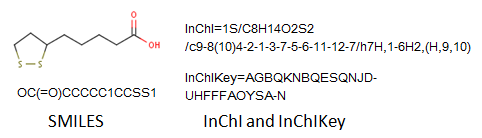
\includegraphics[height=1in]{lipoicacid.png}
\caption{The standard chemical graph illustration together with the
  SMILES, InChI and InChIKey codes for lipoic acid. Note that the
  SMILES is much more human-readable than the others.}
\label{figure:smiles}
\end{figure}

The InChI is now widely used for matching identical chemical
structures, but it is still limited. For example, it cannot
differentiate between certain types of stereoisomers (informally, molecules that are ``3D mirror images'' of each other):
Figure~\ref{figure:cistrans} (in the Appendix) illustrates two
stereoisomers for which the generated InChI is the same.

InChI or other identity-mapping algorithms allow for exact
searching. However, two other practically relevant algorithms for
scientific discovery based on chemical databases are
\emph{substructure searching} and \emph{similarity searching}, which
are required to generalize from the data points contained in a
particular database to other, related molecules. In substructure
searching, the database is searched for a specified wholly contained
part of the structures in the database, while in similarity searching,
the database is searched for structures similar (in some property
space) to a provided search, or query, structure. Chemical search
packages are often implemented and optimized for a given database
technology; for example, the OrChem package is an open source chemical
search package for the Oracle database \cite{rijnbeek2009}.

Graph substructure matching is a variant of \emph{graph isomorphism},
which is widely believed to be computationally
intractable~\cite{cordella2001}. To execute a graph isomorphism search
across a full chemical database of thousands or even millions of
structures is infeasible \cite{Weininger:2011ly}. Speedups can be
obtained via the use of heuristics such as structural
\emph{fingerprints}. Fingerprints encode characteristic features of a
given chemical structure, usually in a fixed-length
bitmap. Fingerprints fall broadly into two categories: structure keys
and hashed keys. In the former, each bit position corresponds to a
distinct substructure such as a \emph{functional group} (a connected set of atoms that affects the characteristics of the chemical reactions of the molecule). Examples
include MACCS and PubChem keys. The latter class are designed such
that substructural patterns are represented as strings and then hashed
to a random bit position. As a result, a given position can encode
multiple substructures. The advantage of such fingerprints is that
they can cover an arbitrarily large collection of substructures such
as ``paths of length $N$,'' or circular environments, and so on. Examples
include ECFPs (Extended Connectivity Fingerprints, which use local topological information) and Daylight fingerprints (which are ``folded'' to optimize information density and screening speed).

Given a binary fingerprint, we can first ``pre-screen'' a database, to
ignore molecules that cannot possibly match the query. This is
achieved by requiring that all bits in a query fingerprint must also
be present in the target fingerprint. Since the target fingerprints
are pre-computed, comparing binary strings can be performed extremely
rapidly on modern hardware. As a result, we apply the actual
isomorphism test only on those molecules that pass the
screen. Fingerprints can also be used to rapidly search databases for
similar molecules, in which case a similarity metric such as the
Tanimoto coefficient is used to compare the query and target
fingerprints. While fast, heuristics have been developed
\cite{Swamidass:2007ve} to further
speed up similarity searches.

\subsection{Linking Molecules to Other Data}
\label{sec:prof-ident}

The preceding section focuses on the choice of representation of
chemical structures. With the profusion of databases that contain
details of small molecules, an emerging problem is the integration of
such databases. Such integration forms the basis of ``systems'' level
investigations of biological systems. A current challenge in
cheminformatics is how to identify ``equivalent'' objects across data
sources. At one level, equivalent compounds can be identified via
canonical structure representations (InChI). But there are other
equivalences beyond structure. For example, compounds may bind to the
same or similar targets; they may be have similar biological function
(say, anti-neoplastic, that is to say, it prevents the development of tumors) and so on. To assess such higher level
characteristics, ontologies and semantic technologies have been
employed, to first, support annotations of chemical systems and
second, enable semantic analyses of chemical systems in conjunction
with other biological systems (such as pathways). A number of
challenges remain in this area - the use of ontologies allows one to
build a semantic network of concepts that links molecules to other
molecules as well as other objects such as targets, genes and
pathways. Open questions include the following.  How does one evaluate similarities in such a heterogenous
network \cite{couto2010}? How does one integrate chemical structure
information with ontologies \cite{hastingsowled2010}? And more
generally, how can we achieve automated inferencing in such
heterogenous linked systems, allowing us to acheive a systems level
understanding of small molecules \cite{Oprea:2007fk}.

\subsection{Expanding Chemical Space}
\label{sec:struct-enum}
Enumerating molecules is a combinatorial problem that has fascinated
chemists, computer scientists and mathematicians alike, for more than
a century. Indeed, many fundamental principles of graph therory and
cominatorics were developed in the context of counting isomers of
paraffin by Cayley, Polya and others. In the 1960's, Lederberg
Dejerassi and others developed algorithms to enumerate structures
based on spectral data, leading to the development of DENDRAL, widely
considered as the first expert system \cite{DENDRAL}.

From a risk reduction point of view efficient methods to enumerate
structures allows us to explore new regions of chemical space (for
example, allowing one to bypass patents), generate structures that
exhibit desired properties, identify molecules matching experimental
data and so on. It is important to realize that chemical space (the
abstract, multi-dimensional space occupied by all possible chemical
structures) is, in principle, infinite. Even considering molecules for
just 30 heavy atoms, the size of this space is on the order of
$10^{60}$ \cite{Bohacek:1996ve}. Any method that purports to enumerate
molecules will inevitably face a combinatorial explosion if
implemented na\"{i}vely.

A key application of structure enumeration is the elucidation of
structures based on spectral data \cite{Kind:2010zr}. This is
especially relevant for the identifying metabolites, small molecules
that are the byproducts of metabolic processes and which provide
insight into the biological state (diseased, fasting, etc.) of an
organism. Ideally, a chemist would gather spectral (mass, LC/MS, etc.)
and the algorithm would provide a list of structures that can give
rise to the observed spectra. Some commercial products such as MOLGEN
(\url{http://molgen.de}) are able to perform this task in a rapid
manner.

Another application of structure enumeration is in the area of Markush
structures and searches \cite{Barnard:1991vn}, where the user
specifies a pattern such as ``\emph{\ldots an aromatic ring with two
  alkyl groups attached to it}.'' Such a pattern is very general: an
alkyl group can be methyl, ethyl or any chain of $n$ carbons and there
are three possible positions for them on the ring. Even in this simple
example there are $3n^2$ possible structures. For more complex
Markushes, there can be billions of possible structures. Clearly,
explicit enumeration is not feasible. Thus one challenge is to devise
methods to search (based on structural or property similarity) through
the implicit enumerated space. A number of commerical vendors such as
Digitial Chemistry and ChemAxon provide toolkits to handle these
problems.

Structure enumeration plays a fundamental role in \emph{molecular
  design} -- the design of compounds (drugs, for instance) that
optimize some physical, chemical, or biological property or activity
\cite{Schneider:2005uq}. A key challenge in this area is to combine
enumeration algorithms with efficient property prediction and is
closely related to methods in predictive modeling of chemical
properties (Section \ref{sec:activity-mining}). This problem is also
termed \emph{inverse QSAR}, where one must devise a set of features
that describe a molecule with a specified property, and subsequently
reconstruct the molecule from those features. As a side note, the
reconstruction of molecules from feature sets is can be considered a
cryptography problem. It is relevant to the pharmaceutical industry,
as it can be necessary to share data on molecules without sharing
explicit structures. Feature sets that allow easy reconstruction of
molecular structures are thus undesirable. A number of workers have
investigated the problem of identify such one-way molecular
descriptors as well as methods to reconstruct molecules from
descriptors \cite{Masek:2008kx} and new methods that generate such
one-way molecular features but still correlate with physicochemical
properties would be invaluable.

While the complexity of molecular graph enumeration remains an open
problem, an alternative to enumerating the space is to sample it
\cite{goldberg1999}. Sampling procedures based on the Metropolis or
the Genetic Algorithms have been developed and used to elucidate
natural compounds from NMR data. It should be noted that even in the
face of the computational complexity of molecular enumeration,
computational chemists have developed and successfully used
enumeration tools to generate large chemical libraries such as GDB-13,
comprising almost a billion chemical structures~\cite{GDB} (but only
considering molecules up to 13 heavy atoms and using only carbon, nitrogen, oxygen, sulfur
and chlorine). Yet, the current enumeration software products do not
generally produce stereoisomers or tautomers; these require specific
enumeration procedures, which are still the subject of investigations
by the cheminformatics community.

Another relevant application of enumeration methods is in the
\emph{generation of chemical reaction networks}. The problem here
consists of enumerating all the possible compounds that can be
produced by applying reaction rules to a set of initial molecules. By
reversing the reaction rules one can also find sets of starting
compounds necessary for producing a given target, known as
\emph{retrosynthesis}. Designing new drugs or chemicals, understanding
the kinetics of combustion and petroleum refining, studying the
dynamics of metabolic networks, applying metabolic engineering and
synthetic biology to produce heterologous compounds (compounds from different species) in microorganisms,
all involve enumeration of reaction networks. As reviewed in Chapter
11 in \cite{faulon2010} several network enumeration techniques have
been developed. However, these techniques generally suffer from a
combinatorial explosion of product compounds. One way to limit the
number of compounds generated is to simulate the dynamics of the
network while it is being constructed and remove compounds of low
concentration. Following that idea, methods have been developed based
on the Gillespie Stochastic Simulation Algorithm (SSA) to compute
on-the-fly species concentrations. Chemical reaction network
enumeration and sampling is an active field of research, particularly
in the context of metabolism, either to study biodegradation, or to
propose metabolic engineering strategies to biosynthesize compounds of
commercial interest. The difficulty with metabolic network design is
that in addition to network generation based on reactions, one also
needs to verify that there are enzymatic events possible for enabling
reactions catalyses (in other words, enzymes must be present to reduce the energy required for some reactions to take place). That additional task requires encompassing both
chemical structure and protein sequence information and the
development of tools that are at the interface between cheminformatics
and bioinformatics.

\subsection{Activity Mining \& Prediction}
\label{sec:activity-mining}


The basis of predictive modeling in cheminformatics is that the
biological activity of a molecule is a function of its chemical
structure. Together with the \emph{similar property principle}
\cite{Johnson:1990qf} (structurally similar molecules will exhibit
similar properties), the goal of any modeling approach is to capture
and characterize the correlations between structural features and the
observed biological activities. Simultaneously, such approaches must
also describe the likelihood of error when using such
models for decision making.  A variety of approaches can be employed
to assess the error in (or conversely, the reliability or confidence of) a
prediction, ranging from statistical approaches to more
empirical approaches such as defining an \emph{applicability domain} -
the region of the input (i.e., chemical structures) that can be
reliably predicted, usually deliniated using some form of similarity
to the training set.

In many cases, the activity of a small molecule is due to its
interaction with a receptor. Traditionally, QSAR \cite{Hansch:1962vn,
  Free:1964ys} approaches do not take into account receptor features,
focusing only on small molecule features, and therefore lose valuable
information on ligand-receptor interactions. As a result, techniques
such as docking (which predicts how molecules fit together), pharmacophore modeling (which predicts the surface features of a molecule) and proteochemometric methods (which predict the interaction between small molecules and proteins)
have been designed to take into account both ligand and receptor
structures. The last method is an example of an extension of
statistical QSAR methods to simultaneous model the receptor and
ligand as first reported by Lapinsh \textit{et  al.}~\cite{lapinsh2001}.

The first step in the predictive modeling of biological activities is
to generate \emph{molecular descriptors} (a.k.a. \emph{features}) that are numerical
representations of different structural features. Here multiple
approaches exist. We can transform molecular graphs into a numerical
vector representation of chemical structures \cite{todeschini2000}, ranging from counts of
elements to eigenvalues of the Laplacian matrix.  Alternatively, we
can compare molecular graphs directly, via \emph{kernel methods}, where a kernel on graphs $G$ and $G'$ provides a measure of how similar $G$ is to $G'$, or a kernel on a single graph compares measures similarities between the graph's nodes. In these
cases, rather than compute vectorial representations, we directly
operate on the graph representations.

Both methods have advantages and disadvantages. The vectorial approach
requires one to identify a subset of \emph{relevant} (to the property
being modeled) descriptors. This is the feature selection problem and
is well discussed in the data mining literature. A kernel approach
does not require feature selection; but now, one faces the problem of
evaluating a data set in a pairwise fashion. Furthermore, one must now
identify an appropriate kernel. This is an important challenge as the
kernel should be selected to satisfy \emph{Mercer's condition} (a well-known mathematical property in machine learning that makes a set of observations easier to make predictions about), and this is
not always possible with traditional cheminformatics based kernels
(such as a multiple common substructure based kernel). These
challenges can make kernel based methods prohibitive on very large
datasets.

Having settled on a numerical representation and a possible class of
model types, one must address the goal of the model. Are we
looking for pure predictive power, with no interest in any explanatory
features? Or are we more interested in decent predictive power, but
also some explanation as to why a molecule is predicted as toxic or
non-toxic, for example. The former scenario is common in virtual
screening settings, where we require a high degree of accuracy and fast
predictions, but do not really care why one molecule is active
and another inactive. These types of models can be black boxes (neural
networks) and algorithmic models \cite{Breiman:2001fk} (random
forests). The latter scenario is more common in exploratory and
optimization settings, where we hope that the output of the model will
guide us in chemical modifications to improve the property being
modeled.  In this case, we need to understand the effect of a
certain structural feature on the observed potency and expect that the
model will provide insight. These types of models are generally
distributional in nature (such as linear regression and Partial Least Squares) though
some algorithmic approaches such as random forests can provide insight.

Having chosen a modeling approach, a vital question is that of model
reliability which is closely tied to the concept of model
applicability -- the question of when the prediction of the model for
a new object is reliable. This issue has grown in importance with the
increasing use of predictive models in regulatory settings. A
misprediction (due to the model not being applicable to a certain class
of inputs) can have significant financial repercussions. A variety of
methods have been developed that attempt to characterize the domain of
a model. These methods not only determine whether models are
applicable, but can also be used for deciding if additional biological
experiments are required for reducing the prediction error on certain
compound classes.

One of the key challenges faced by predictive modeling is the fact
that small molecules are not static and do not exist in
isolation. Traditionally, predictive models have focused on a single
structure for a small molecule and have ignored the role of the
receptor (in receptor-mediated scenarios). Yet, small molecules can
exist in multiple tautomeric forms and usually in multiple
conformations. As a result, enhancing the accuracy of predictions
ideally will require that the 3D geometries of that molecule be taking into account and, as
far as possible, take into account the receptor
simultaneously. Multi-conformer modeling has been addressed in the
4D-QSAR methodology described by Hopfinger and co-workers
\cite{Albuquerque:1998ys}.  Recent techniques such as
\emph{multiple-instance learning} could also be applied to the
multi-conformer problem.

With the advent of high-throughput screening technologies, large
libraries of compounds can be screened against multiple targets in an
efficient manner. Such panel assays provide a broad, systems-level
view of small molecule activities.  Models developed on such data
afford us the opportunity to identify targets, characterize off-target
effects and so on. However, most approaches to this problem tend to
develop multiple individual models \cite{Chen:2010zr}, leading to
multiple, independent predictions for a given input molecule.
Instead, one could imagine an approach that takes into account the
covariance structure of the multiple observed activities and the
structural descriptors within a single model. Such an approach could
lead to more robust predictions for panel assays (that is, which battery of tests would be most useful to perform). Finally, this
approach also better reflects clinically relevant compound
profiles~\cite{kuhn2010} and the ``personalized medicine'' concept
(\emph{e.g.}, drug-drug interaction profiles).

\subsection{Knowledge Management}
\label{sec:knowledge-management}

The relevance of scientific knowledge management is increasing not
only for reducing the risk in current research, but also for enabling
new collaboration/innovation opportunities with internal partners and
a rapidly growing number of external/public partners. In
cheminformatics and chemistry, scientists already switched years
ago from paper lab-notebooks to online collaboration platforms, called
ELNs (Electronic Lab Notebooks). So, what were the drivers behind
chemists, and companies, adopting ``Enterprise 2.0,'' a social online
collaboration culture?

Before the year 2000, many chemists were still using paper
lab-notebooks, multiple compound registration, and search
tools. The overall architecture was too inflexible to
adopt to fast changing data standards, scientists spent too much time
with administrative work, chemical data quality was inconsistent, an
alignment with other working groups was inefficient (\emph{e.g.}, for
running analytical experiments). Legal disputes would require manual
searches through many paper lab notebooks and data synchornization was
painful, hampering large scale collaborations.

%  Now, chemists prefer ELNs, because they can run
% searches in the data across the organization. This does not only allow
% to find experts faster, but also allows access to highly trusted data
% with approved quality workflows. Since this also gives access to
% analytical and legal data directly every new ELN release is aiming at
% increasing the integration of scientific and business workflows for
% reducing the risk due to irrational or bounded-rational decision
% making and increasing decision making efficiency.

While ELNs technically existed as long ago as the 1990s, chemists
adopted their use in large numbers in 2004 and 2005, and the market is
still growing~\cite{ELNstatus}. As one report notes, ``The initial
drive for the development of ELNs came from the field of chemistry,
perhaps driven by the early adoption by chemists of computer
technologies \ldots The pharmaceutical industry shifted from a
position of `if we get an ELN' to `when we get an
ELN'.''~\cite{ELNstatus}. The growth of the use of ELNs has been
driven by many factors including ease of use (rapid searches across
organization-wide data sources, easy sharing of domain knowledge) and
regulatory compliance (timestamped experimental data, experiment and
data approvals and quality control information). Given that any experiment could
become the core of a patent filing, ELNs allow organizations to define
and implement audit trails in a standardized and efficient fashion.

At this point, ``electronic lab notebooks have replaced the
traditional paper lab book across the pharmaceutical industry,'' but
are not yet common in academia, because of their high
cost~\cite{WavingGoodbye}.  It is worth mentioning that chemistry is
traditionally a field where many people have been used to huge
bookshelves of reactions and compounds. Chemists changed to online
ELNs not only to increase efficiency, but also because it allowed easy
collaboration with trusted colleagues. Third party paper catalogs and
academic publications proved to be inefficient, and even more
critically, they did not take compounds of trusted colleagues into
account. Overall the change of management to ELNs, similar to
``Enterprise 2.0,'' required delivering on the promise to increase
interconnectivity, and to improve collaboration opportunities.  The
leading players in this area include CambridgeSoft's E-Notebook and
Accelrys' Symyx Notebook, but there are at least 35 different
companies producing ELNs as of February 2011~\cite{ELNreview}, for use
in chemistry, biology, quality control, and other research.  Another
knowledge management tool specifically for chemists is the web-based
service Reaxys, founded in 2009, whose company goal is to provide ``a
single, fully integrated chemical workflow solution.''

However, the future still leaves many challenges ahead. Using
external/public databases with chemical and bioactivity data remains a
challenge due to differences in identifiers, synchronization, curation
\& error correctin mechanisms and efficient substructure and
similarity search within complex data types (compounds). A
collaboration with external parties, e.g. contract research, poses
other problems including compound duplication and efficient data
synchronization. If external partners are small they often do not even
have sufficient IT resources themselves and thus rely on external
services. Cloud services could help not only to provide a service
infrastructure for all parties involved, but also to provide the
required private/public access toolbox. Furthermore, there are still
many data sources not being indexed properly: chemistry patents are
often cryptic and chemical image and text mining remains a challenge
(albeit, currently being addressed in academia and industry
\cite{Jessop:2011fk,Sayle:2009uq}). The closed CAS (Chemical Abstract
Service) is a highly trusted source, and public chemistry and
bioactivity space has to improve quality and interconnectivity to
compare with it. Efforts like ChEMBL and PubChem-BioAssay are on the
right track. Still, improving data quality and standards between
public and closed sources will be absolutely critical for ensuring
constant growth, usage, and collaboration scenarios between private
and public parties.

\section{Support for the Development of Novel Algorithms}
\label{sec:development-support}

For researchers interested in the development of new algorithms in the
field, a software library that handles chemical structures and related
data is essential. A wide variety of such chemical toolkits are
available, both commercial (which may offer free academic
licenses) and Open Source.

Due to the importance of cheminformatics to the pharmaceutical
industry in particular, numerous commercial vendors provide libraries,
applications and database cartridges to handle a wide variety of
needs including Accelrys, BioSolveIT, ChemAxon, Chemical Computing Group,
Daylight, Open Eye, Schrodinger, Tripos, and Xemistry. More recently
there has been a growth in the development of Open
Source cheminformatics software, and this presents opportunities for
the rapid development and implementation of novel algorithms which can
build on the existing Open Source ecosystem. In this article we do not debate the
arguments for and against Open Source; we focus on Open Source
tools simply because this ensures that a reader will be able to explore
cheminformatics problems with a minimum of encumbrances.

The extent of open-source software in cheminformatics has somewhat
lagged behind related fields such as bioinformatics, partly due to the
existence of a lucrative pharmaceutical market for proprietary
software. However, in recent years there has been a rise in the amount
of open-source cheminformatics software. One contribution to this has
been the Blue Obelisk group~\cite{BlueObelisk2011}
(\url{http://blueobelisk.org}) of chemists, who have worked together
to create interoperable open-source chemistry software (among other
activities). Now there are a number of Open-Source chemical toolkits
available including the Chemistry Development Kit
(CDK)~\cite{steinbeck2003}, Open Babel~\cite{openbabel2011}, RDKit and
Indigo. These toolkits are written in Java or C++ (though toolkits
written in the latter invariably have bindings to a variety of
languages). Such toolkits are used, for example, to read/write
chemical file formats, manipulate chemical structures, measure
similarity of molecules, search for substructures, and generate 2D
diagrams. The underlying algorithms used include graph algorithms
(e.g. maximal common substructure, canonical labelling of graphs),
geometrical methods (e.g. Kabsch alignment) and vector manipulation
(e.g. converting coordinates in various systems, 3D structure
generation). As well as being of direct use to practising
cheminformaticians in their day-to-day work, many applications have
been developed that rely on these toolkits to handle chemical data;
for example, the molecular viewer Avogadro
(\url{http://avogadro.openmolecules.net}) uses Open Babel, while the
molecular workbench Bioclipse~\cite{Bioclipse2} uses the CDK.

The various toolkits have many features in common and at the same time
have certain distinguishing features. For example, the CDK implements
a large collection of molecular descriptors. On the other hand, Open
Babel has robust support for 3D structure generation and optimization
and supports the interconversion of a huge number of chemical file
formats. Table~\ref{tab:features} (in the Appendix) compares features
offered by the open-source toolkits currently available.  Given that
there is ample scope for software engineering (algorithm
implementation, code quality and analysis, build systems etc), both
the CDK and Open Babel are open to new contributions. Both are driven
via public, active mailing lists and public issue tracking systems.

It is important to note that certain challenges faced by nearly all
cheminformatics toolkits stem from the graph representation of
chemistry. This representation, while succinct and amenable to
computation, is only an approximation of reality -- and edge cases
abound. Existing areas of interest are enumeration of colored graphs,
taking into account symmetry, and symmetry detection itself, which not
merely derives from the chemical graph, but typically also from the 3D
geometry of the chemical. It is important to realize that although
chemical representations have increased in sophistication over the
years, many chiral molecules cannot be satisfactorily handled by
current representation systems. Perhaps a more challenging aspect is
that the chemical representation of a molecule really needs to capture
non-static graphs, in order to take into account delocalisation and
the tautomeric phenomena molecules can undergo in practice.

Of equal importance to the development of new algorithms is freely
available data on which to train and test new methods. As has been
noted, recently large structure and bioactivity data collections have
become available. As a result, this enables much more robust
validation of cheminformatics methodologies as well as large scale
\emph{benchmarking of algorithms}. The latter is especially relevant
for the plethora of data mining techniques that are employed in
cheminformatics. At this point, the nature of Open Data focuses
primarily on structure and activity data types. On the other hand,
there is a distinct lack of textual data (such as journal articles)
that are ``Open'' in nature. While PubMed abstracts serve as a proxy
for journal articles, text mining methods in cheminformatics are
hindered by not being able to mine the full text of many scientific
publications.  Interestingly, patent information is publicly
accessible (cf. Google Patents) and represents an excellent resource
to support these types of efforts.

%
\section{Conclusions}
\label{sec:conclusions}
Cheminformatics, the computer science of chemical discovery, is an
industrial and academic discipline with roots dating back to the 19th
century and flowering in the 1960s with the advent of modern computing
technologies. While many key cheminformatics techniques have been
available in the literature since the 1960's, the bulk of
cheminformatics tools and implementations have been proprietary. In
addition, most data sources of chemical information have been
proprietary (usually with restrictive licensing policies) until
recently. There are many reasons for this, primarily revolving around
issues of profits, competitive intelligence and intellectual property,
which are relevant to the pharmaceutical as well as other chemical
industries. This is in contrast to much of bioinformatics, where the
data and tools have been freely available since the inception of the
field. One could argue that the outcomes from cheminformatics methods
and software have a more direct impact on profits, in terms of
identifying lead like compounds and improving properties of drug
candidates. In contrast, much bioinformatics software is employed in
upstream areas such as target identification (finding molecules that react well with the molecule under consideration).  While certainly
important, this type of research is not as directly related to
possible profits as an actual small molecule.

Furthermore, chemical data (structure, activity information etc.) is
harder to acquire and when done on large scales can be extremely
intensive in terms of time and effort. Thus much of it has been
proprietary. Whereas a lot of bioinformatics data (sequences for
example) are much easier to obtain. While both fields have theoretical
components, it is possible that the free availability of large amounts
of data in bioinformatics drove the development of publicly
available tools to handle it. In contrast, the proprietary nature of
chemical data would imply that tools to process and analyze that data
were of interest primarily to the owners. As a result, the incentive
to make cheminformatics software public has been low and since the
users of it were primarily industrial, commercial software was the
norm.

Of course, with the advent of systems biology and its large amounts of
heterogenous data and wide array of (possibly profitable) commercial
applications, this may change. Indeed, in biology, the
requirement to consider small molecules in the context of larger
biosystems implies that cheminformatics and bioinformatics will both
be required to tackle future problems.

As we enter the second decade of the 21st century, the cheminformatics
landscape is rapidly shifting.  There now exist free-of-charge
open-source cheminformatics toolkits, applications and open databases
with tens of millions of compounds and containing valuable
experimental bioactivity data. Modern experimental techniques such as
high throughput sequencing have made the generation of large amounts
of structure-activity data much more accessible.  We believe the
prospects for academic and industrial collaboration between chemists
and computer scientists are bright, and we would like to encourage
more computer scientists to participate in cheminformatics research.

There is an admittedly steep learning curve, as significant domain
knowledge is required to attack many problems in cheminformatics due
to the underlying chemistry of the systems being studies. Indeed, many
issues faced by chemists are often detailed and subtle and do not
admit as clean an abstraction as ``algorithms on a string'', the way
many bioinformatics algorithms can be abstracted into a computer
science framework.  As a result, while one can certainly make
significant contributions to cheminformatics by just considering
structures as graphs, one is limited to somewhat abstract
problems. Keeping in mind that cheminformatics is fundamentally a
practical field that serves to help and advance experimental
chemistry, the key challenges require an understanding of the
underlying chemical systems. 
%One could certainly study for a degree in chemistry. Alternatively one could collaborate with a chemist or cheminformatics practitioner.

Nevertheless, because of the increasing availability of tools and
data, the barrier to entry for non-chemists and non-cheminformaticians
is significantly lower than it was a decade ago. Many questions that benefit from computer
science can now be comprehensively tackled: for a theorist,
graph-theoretic questions of three-dimensional enumeration; for a
database designer, more effective search algorithms and ontologies;
for a practical programmer, expansion of the many open-source
cheminformatics projects.  If more chemists think algorithmically, and
more computer scientists think chemically we are much better
positioned taking not only ``simple'' chemicals into account (only one
identifier and isomer possible per molecule), but also their complex
relationships, transformations, and combinatorial challenges.

\section{Acknowledgements}
We would like to thank Danny Verbinnen for sharing his insights into
ELNs.  This article was written while A. Sterling was visiting the
Department of Electrical Engineering and Computer Science,
Northwestern University, supported in part by NSF grant
CCF-1049899. A. Bender thanks Unilever for funding.

\bibliographystyle{abbrv}
\bibliography{paper}

\appendix

\section{Glossary of Terms}
\begin{itemize}
\item \textit{Bioassay} - A system measuring the biological activity of a chemical compound on a particular
    biological assay (with all its parameters).
\item \textit{Biodegradation} - is the chemical dissolution of materials by bacteria or other biological means.
\item \textit{Conformation and conformational isomerism} - In chemistry, conformational isomerism is a form of
    stereoisomerism in which the isomers can be interconverted exclusively by rotations about formally single
    bonds.
    Single possible states of compounds are called conformers.
\item \textit{Ligand (biochemistry)} - a substance that binds to a protein.
\item \textit{Ligand (coordination chemistry)} - an atom, ion, or functional group that donates one or more of its
    electrons through a coordinate covalent bond to one or more central atoms or ions.
\item \textit{Mass spectrometry} - Mass spectrometry (MS) is an analytical technique that measures the
    mass-to-charge ratio of charged particles. It is used for determining masses of particles, for determining the
    elemental composition of a sample or molecule, and for elucidating the chemical structures of molecules, such
    as
    peptides and other chemical compounds.
\item \textit{Protonation and protonation state} - In chemistry, protonation is the addition of a proton (H$^+$) to
    an atom, molecule, or ion. The different states (different number of H$^+$ or on different atoms) are called
    protonation states for a molecular compound (e.g. de-protonated, mono-protonated, di-protonated, or any
    variations of those states).
\item \textit{QSAR} - Quantitative Structure-Activity Relationships; methods to relate the structure and the
    biological activity of a chemical structure in a quantitative manner.
\item \textit{Reaction catalysis} - Catalysis is the change in rate of a chemical reaction due to the participation
    of a substance called a catalyst.
\item \textit{Receptor (biochemistry)} - in biochemistry, a protein molecule that receives and responds to a
    neurotransmitter, or other substance.
\item \textit{Regulatory authorities} - In the US the Food and Drug Administration (FDA) is responsible for
    protecting and promoting public health through the regulation and supervision of e.g. dietary supplements,
    prescription and over-the-counter pharmaceutical drugs (medications), vaccines, biopharmaceuticals, medical
    devices, and many other health related items. The European Medicines Agency (EMA) is a European agency for the
    evaluation of medicinal products.
\item \textit{SMARTS} - SMiles ARbitrary Target Specification \\(SMARTS) is a language for specifying substructure
    patterns in molecules
\item \textit{Stereoisomer/stereoisomerism} - Stereoisomers are isomeric molecules that have the same molecular
    formula and sequence of bonded atoms (constitution), but that differ only in the three-dimensional orientations
    of their atoms in space.
\item \textit{Tautomerism} - Tautomers are isomers (same molecular formula but different structural formula) of
    organic compounds that readily interconvert by a chemical reaction called tautomerization.
\end{itemize}
%
\section{Additional Figure and Tables}
%
\begin{table*}
\begin{tabular}{|l|l|l|} \hline
\textbf{Property} & \textbf{Requirement} & \textbf{Potential of Cheminformatics Approaches} \\ \hline
\multicolumn{3}{|l|}{\textbf{Research Stage}} \\ \hline
\multirow{3}{*}{Bioactivity} & Compound is active & \textsc{High} -- computer models can often predict \\
& in \emph{in vitro} (``test tube'')
studies &  which compounds are bioactive, \\
&& the so-called \emph{virtual screening} approaches \\ \hline
\multirow{3}{*}{Solubility} & Compound is soluble  & \textsc{High} -- computer models can often predict \\
& at effective concentration & which compounds are insoluble, \\
&& decreasing the need for experimental testing \\ \hline
\multirow{3}{*}{No Obvious Toxicity} & No known ``toxicophores''  & \textsc{High} -- approaches such as substructure
searching \\
& contained within molecule & are routinely applied to remove
chemical structures \\
&& with functional groups that
are known to be toxic \\ \hline
\multirow{3}{*}{Selectivity} & Compound does not modulate  & \textsc{Medium} -- \emph{in silico} approaches can often make
guesses  \\
& other than  & which proteins are modulated by a
molecule, but the \\
& the intended protein
target & precise prediction of
bioactivity profiles remains a challenge \\ \hline
\multicolumn{3}{|l|}{\textbf{Development Stage (All of the above, plus...)}} \\ \hline
\multirow{3}{*}{Efficacy} & Compound is not only
active
& \textsc{Low} -- bioinformatics approaches can partially
be used  \\
 & in the test tube, but also & to anticipate whether modulation of a
particular protein  \\
in Animal/Human Models & in the
organism  & shows an effect in humans via pathway modeling\\ \hline
\multirow{3}{*}{Safety in} & Compound exhibits
tolerable & \textsc{Low} -- bioinformatics approaches can partially
be used \\
& side effects in
animal
models & to anticipate safety concerns in
humans, \\
Animal/Human Models & and/or humans & however experimental confirmation is
required \\ \hline
\multirow{4}{*}{Bioavailability} & Compound gets
dissolved & \textsc{Medium} -- cheminformatics models for
bioavailability  \\
& in the
gastrointestinal tract & can be generated, however due
to the complexity  \\
& and it is absorbed into
the  & of the process they are in
many cases  \\
& bloodstream & not sufficiently reliable for practical
use \\ \hline
\multicolumn{3}{|l|}{\textbf{Marketed Drug (All of the above, plus...)}} \\ \hline
\multirow{3}{*}{Cost of Synthesis} & The compound can be
 & \textsc{Medium} -- some cheminformatics approaches
exist \\
& synthesized at a  & that can estimate the difficulty of \\
& reasonable cost & synthesizing a particular chemical structure \\ \hline
\multirow{2}{*}{}Better Efficacy & The compound has & \textsc{Medium} -- the profile of the final product will
determine  \\
than Competitor Products & a market advantage & the particular advantage of the drug
in the market \\ \hline
\multirow{4}{*}{} & Patients with a disease & \textsc{Medium} -- business decisions are quite relevant \\
Existence of  & treated by the drug exist & when drugs are developed in private pharmaceutical \\
Relevant Market Need   & and they possess the means  &  companies (but often to a lesser extent \\
& to buy the drug &  in government-owned pharmaceutical research laboratories) \\  \hline
\end{tabular}
\caption{Some of the properties potential drug candidates need to have to be considered as ``promising,'' either in the different research and development stages, as well as a drug that is finally admitted to the market. Note that the particular requirements are also heavily project-dependent, and that also in cases where cheminformatics approaches can be employed in drug design an experimental confirmation of the prediction is required -- the computer can hence decrease the experimental burden, but not replace it altogether.}
\label{table:properties}
\end{table*}
%
\begin{table*}
  %\onehalfspacing
  \centering
  \begin{tabular}{lcccc}  \hline
    \textbf{Feature} & \textbf{CDK} & \textbf{OpenBabel} &
    \textbf{RDKit} & \textbf{Indigo}\textsuperscript{1} \tabularnewline \hline
    License & LGPL & GPL & new BSD & GPL or commercial \tabularnewline
    Language & Java & C++ & C++ & C++ / Python \tabularnewline
    SLOC\textsuperscript{2} & 188,554 & 194,358 & 173,219 & ? \tabularnewline
    Structure-based Fingerprints & \lots\textsuperscript{3} & \lots & \lots & yes \tabularnewline
    %\ \ \ Substructure & \lots & \lots & \lots \tabularnewline
    Support for multiple chemical file formats & \little & \lots & \least & \little \tabularnewline
    %Aromaticity models & \least & \least & \least \tabularnewline
    %Stereochemistry & \least & \little & \lots \tabularnewline
    Canonical labeling of graphs & \lots & \lots & \lots & yes \tabularnewline
    Calculation of molecular descriptors & \lots & \least & \lots & no \tabularnewline
    %2D coordinate generation & \lots & \none & \lots & no \tabularnewline
    3D coordinate generation & \least & \lots & \lots & no \tabularnewline
    2D depictions & \lots & \little & \lots & \little \tabularnewline
    Generation of conformational isomers & \none & \least & \least & no \tabularnewline
    %Rigid alignment & \lots & \lots & \lots \tabularnewline
    SMARTS searching/matching & \lots & \lots & \lots & yes \tabularnewline
    %Pharmacophore searching & \little & \none & \lots \tabularnewline
    Chemical reaction enumeration & no & no & no & yes \tabularnewline
    \hline
    \multicolumn{5}{l}{1. Indigo is a new toolkit (published late 2010), and we have not investigated its features in depth.} \\
    \multicolumn{5}{l}{2. Source Lines of Code as measured by the tool \emph{sloccount} (\url{http://www.dwheeler.com/sloccount/}).} \\
    \multicolumn{5}{l}{The count includes all source files, in any language, for the
  project. In addition, only the trunk} \\
    \multicolumn{5}{l}{for each project was considered.  We did not count Indigo's lines of code.} \\
    \multicolumn{5}{l}{3. More checks indicates more complete implementation of a feature.} \\
  \end{tabular}
  \caption{Cheminformatics features provided by open-source toolkits.}
  \label{tab:features}
\end{table*}

\begin{figure}
\centering
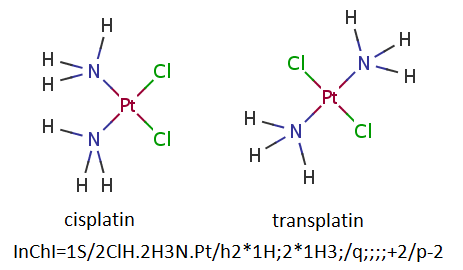
\includegraphics[height=1.3in]{platins.png}
\caption{The generated InChI is the same for the stereoisomers cisplatin and transplatin.}
\label{figure:cistrans}
\end{figure}
%
\begin{figure}
\centering
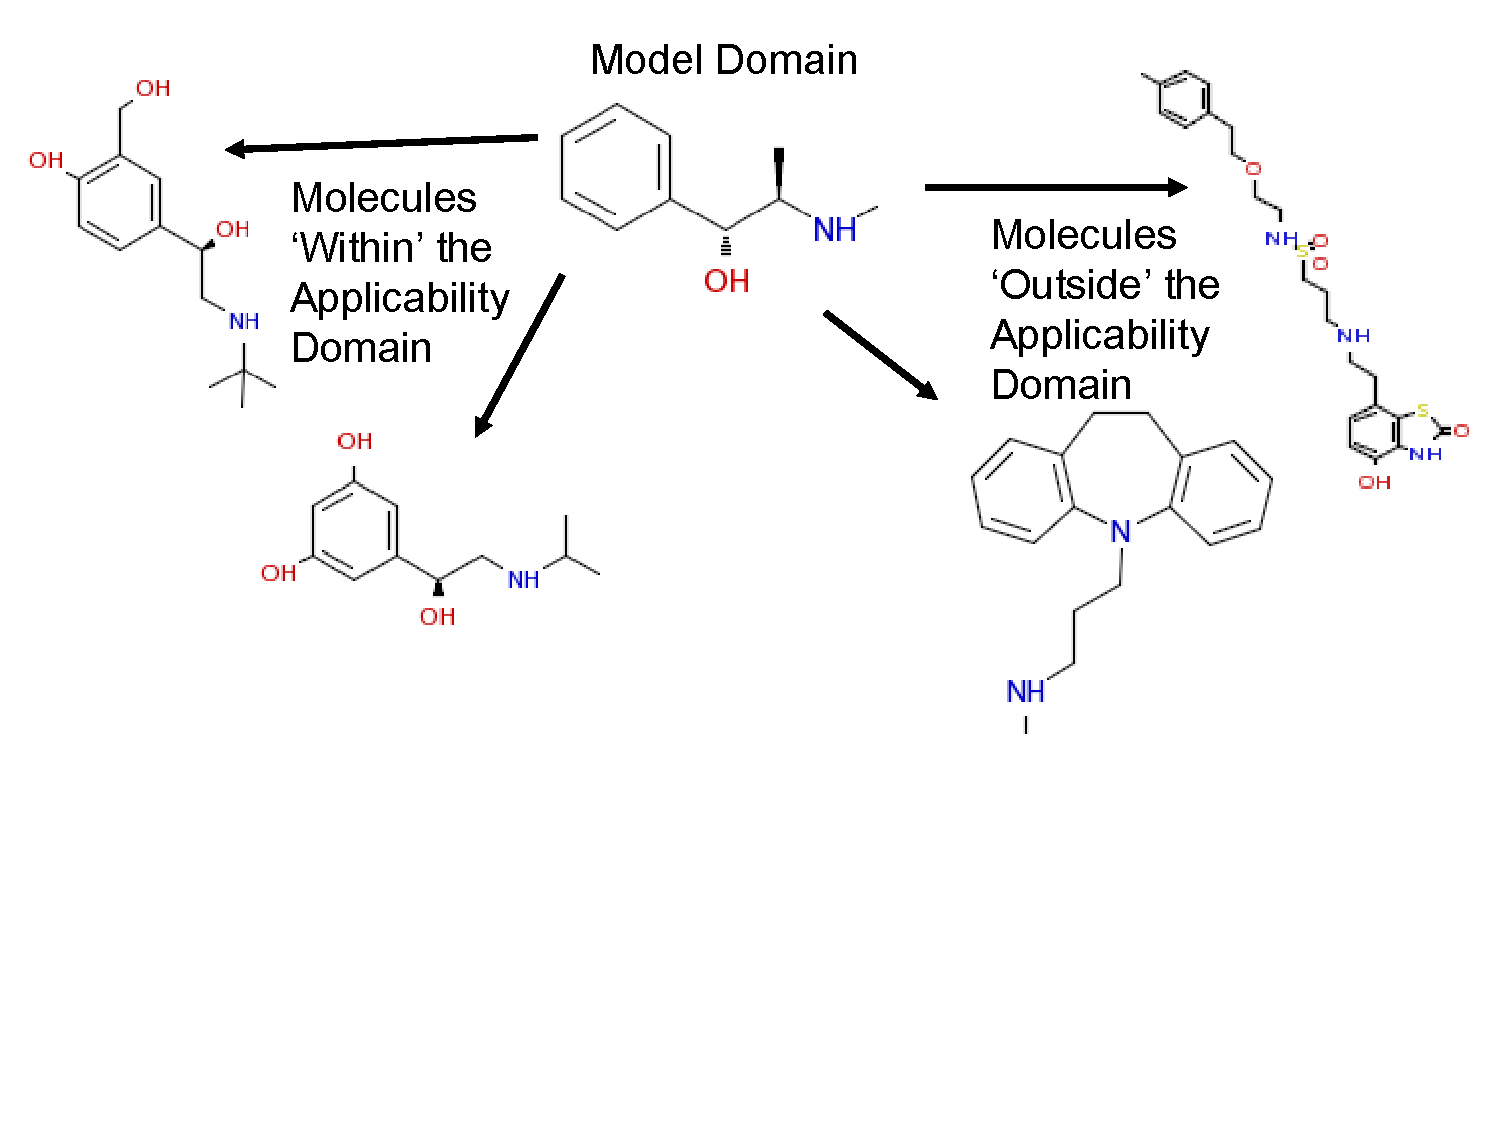
\includegraphics[height=2in]{CACM_ApplicabilityDomain.pdf}
\caption{Illustration of the ``Applicability Domain'' concept. In order to estimate whether model predictions are reliable, it is crucial to define areas of ``chemical space'' where the model is applicable, and where it is not. In this case, the ``model domain'' includes the molecule at the top. The (relatively similar) molecules to the left are likely to be included in the Applicability Domain of the model, while the (more dissimilar) molecules to the right are likely located outside this domain, hence the generated model is probably not applicable.}
\label{figure:applicability-domain}
\end{figure}
%
\end{document}
